\begin{figure}[!htb]
  \centering
  \begin{subfigure}[b]{0.2\textwidth}
    \centering
    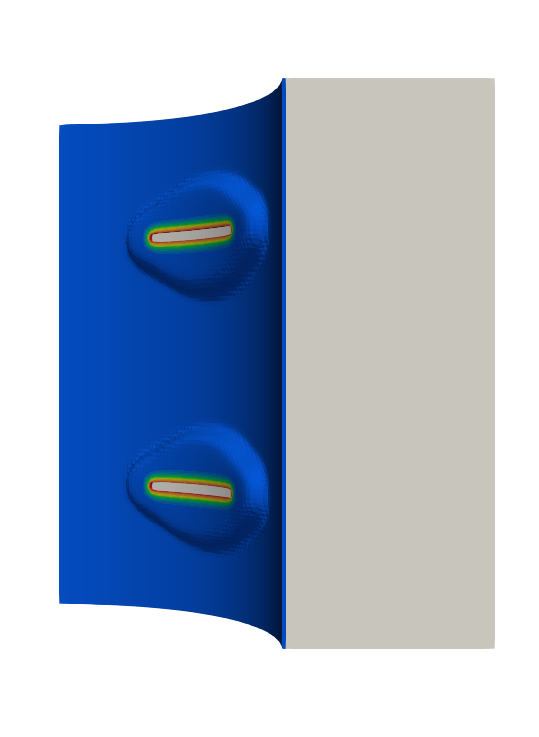
\includegraphics[width=\textwidth]{Chapter5/figures/spallation/seed_d_4}
    \caption{0 hour}
  \end{subfigure}
  \begin{subfigure}[b]{0.2\textwidth}
    \centering
    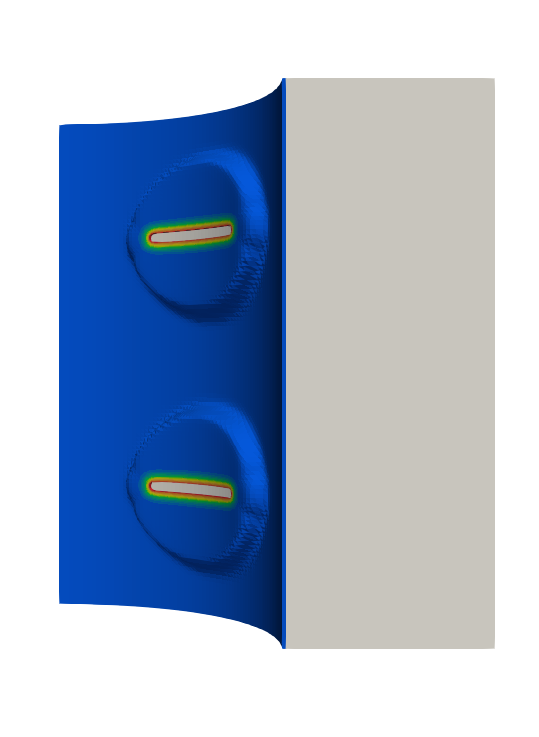
\includegraphics[width=\textwidth]{Chapter5/figures/spallation/seed_d_5}
    \caption{1 hour}
  \end{subfigure}
  \begin{subfigure}[b]{0.2\textwidth}
    \centering
    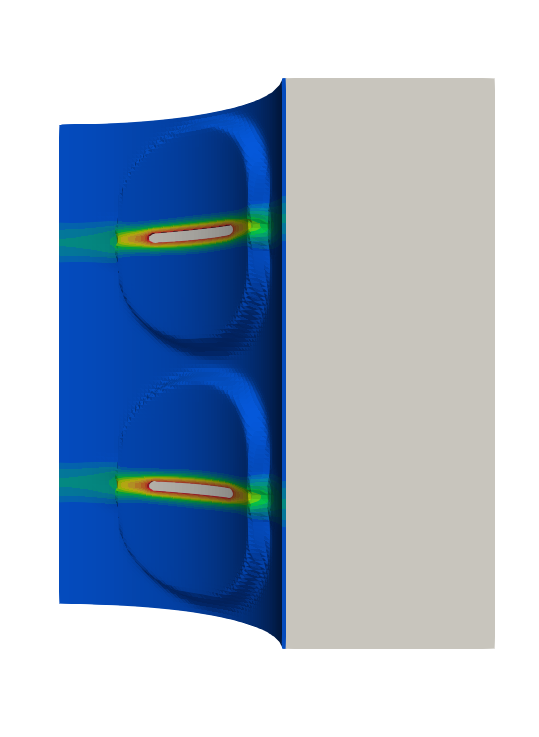
\includegraphics[width=\textwidth]{Chapter5/figures/spallation/seed_d_6}
    \caption{2 hours}
  \end{subfigure}
  \begin{subfigure}[b]{0.2\textwidth}
    \centering
    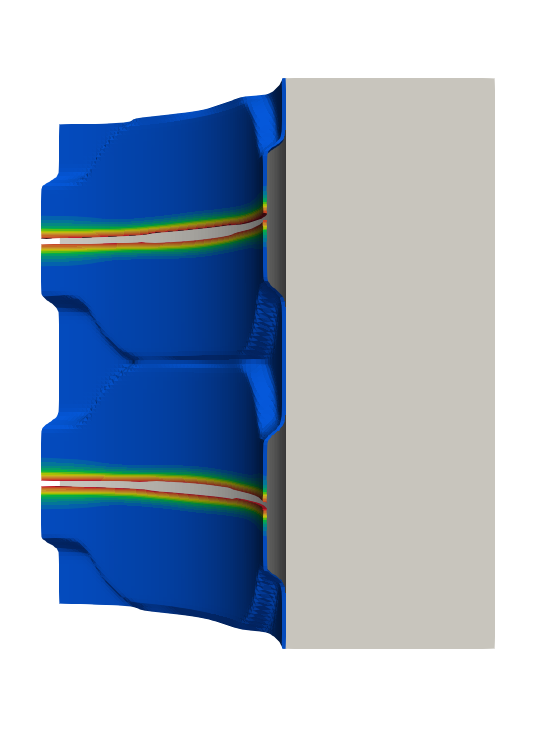
\includegraphics[width=\textwidth]{Chapter5/figures/spallation/seed_d_7}
    \caption{3 hours}
  \end{subfigure}
  \begin{subfigure}[b]{0.1\textwidth}
    \centering
    \caption*{$d$}
    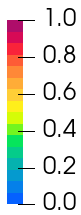
\includegraphics[width=0.6\textwidth]{Chapter5/figures/spallation/colorbar_d_seed}
    \vspace{4em}
  \end{subfigure}
  
  \begin{subfigure}[b]{0.2\textwidth}
    \centering
    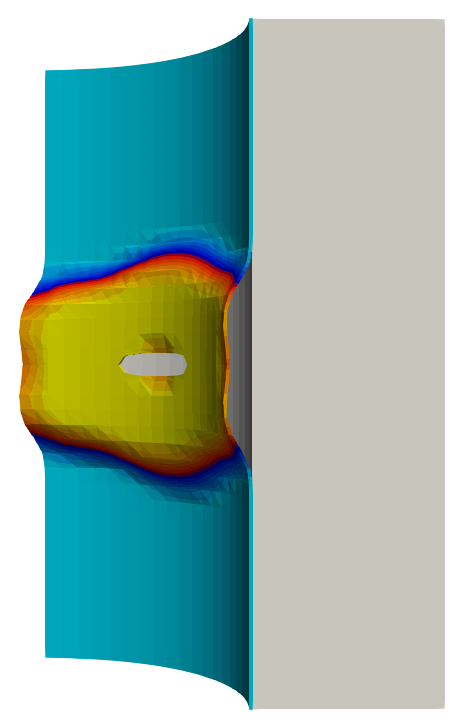
\includegraphics[width=\textwidth]{Chapter5/figures/spallation/seed_c_4}
    \caption{0 hour}
  \end{subfigure}
  \begin{subfigure}[b]{0.2\textwidth}
    \centering
    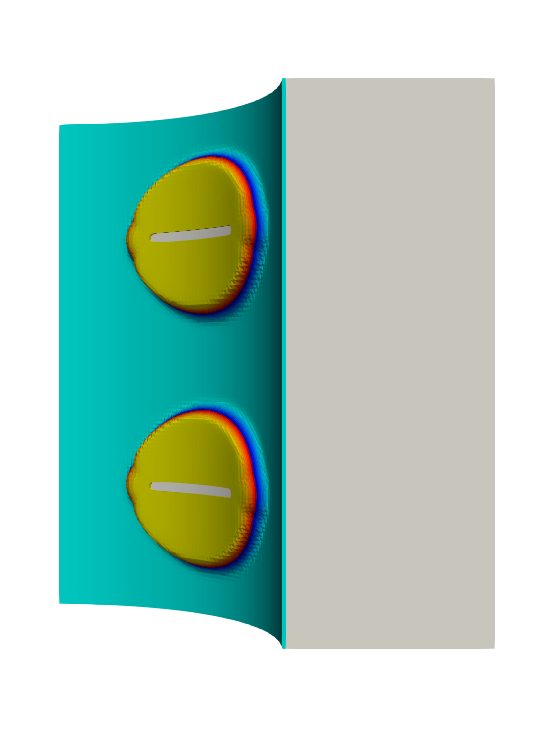
\includegraphics[width=\textwidth]{Chapter5/figures/spallation/seed_c_5}
    \caption{1 hour}
  \end{subfigure}
  \begin{subfigure}[b]{0.2\textwidth}
    \centering
    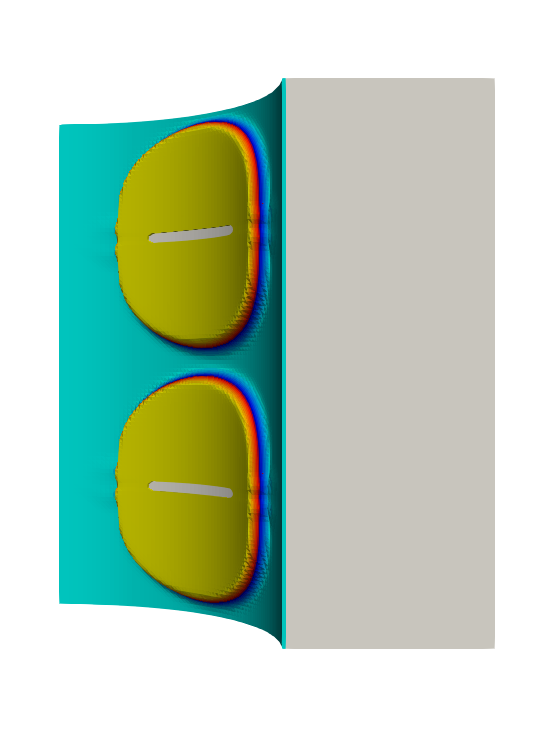
\includegraphics[width=\textwidth]{Chapter5/figures/spallation/seed_c_6}
    \caption{2 hours}
  \end{subfigure}
  \begin{subfigure}[b]{0.2\textwidth}
    \centering
    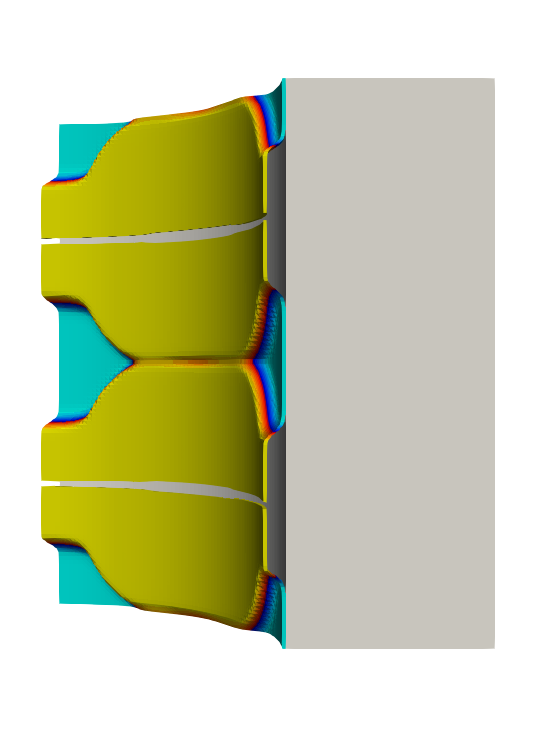
\includegraphics[width=\textwidth]{Chapter5/figures/spallation/seed_c_7}
    \caption{3 hours}
  \end{subfigure}
  \begin{subfigure}[b]{0.1\textwidth}
    \centering
    \caption*{$c$}
    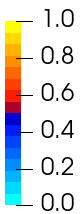
\includegraphics[width=0.6\textwidth]{Chapter5/figures/spallation/colorbar_c_seed}
    \vspace{4em}
  \end{subfigure}
  
  \begin{subfigure}[b]{0.2\textwidth}
    \centering
    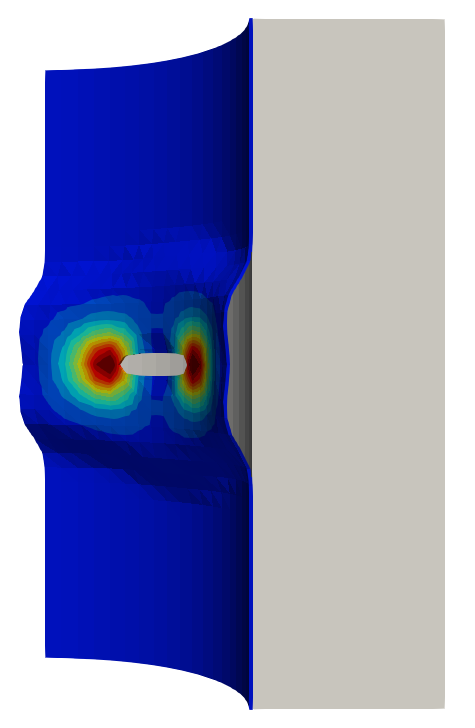
\includegraphics[width=\textwidth]{Chapter5/figures/spallation/seed_ep_4}
    \caption{0 hour}
  \end{subfigure}
  \begin{subfigure}[b]{0.2\textwidth}
    \centering
    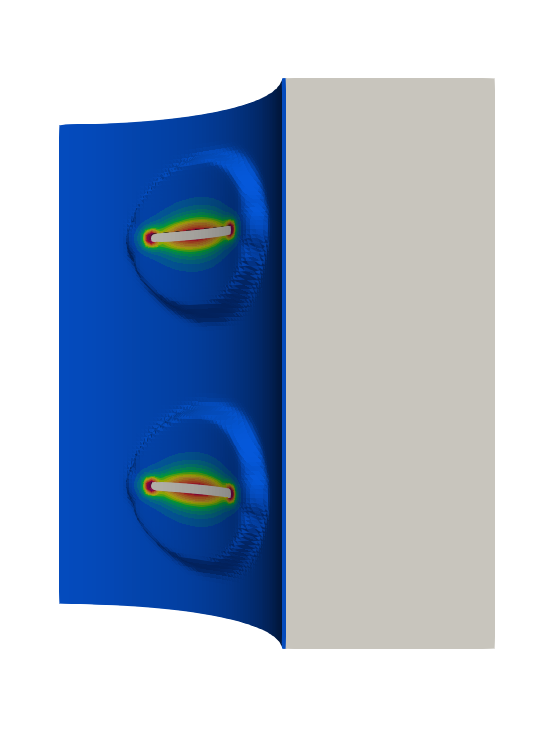
\includegraphics[width=\textwidth]{Chapter5/figures/spallation/seed_ep_5}
    \caption{1 hour}
  \end{subfigure}
  \begin{subfigure}[b]{0.2\textwidth}
    \centering
    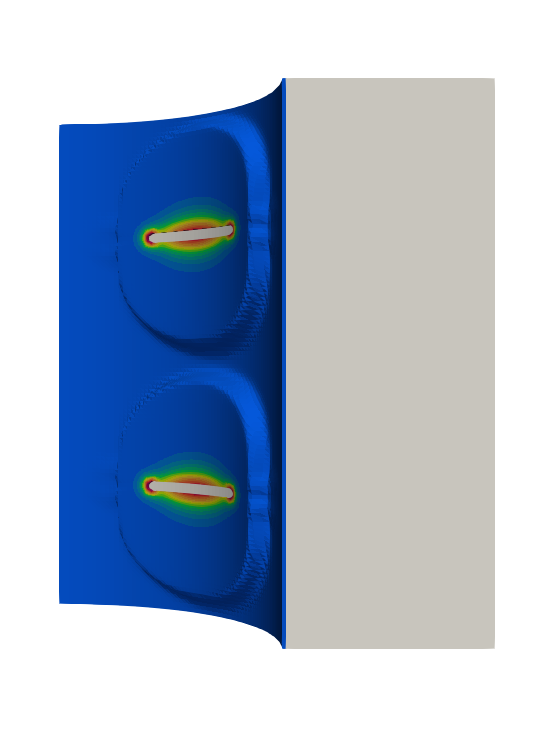
\includegraphics[width=\textwidth]{Chapter5/figures/spallation/seed_ep_6}
    \caption{2 hours}
  \end{subfigure}
  \begin{subfigure}[b]{0.2\textwidth}
    \centering
    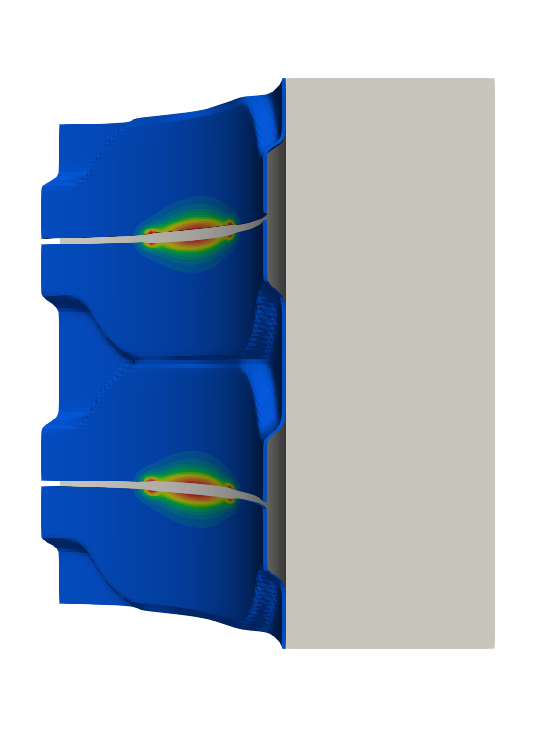
\includegraphics[width=\textwidth]{Chapter5/figures/spallation/seed_ep_7}
    \caption{3 hours}
  \end{subfigure}
  \begin{subfigure}[b]{0.1\textwidth}
    \centering
    \caption*{$\ep$}
    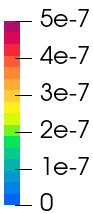
\includegraphics[width=0.6\textwidth]{Chapter5/figures/spallation/colorbar_ep_seed}
    \vspace{4em}
  \end{subfigure}
  \caption[Simulation of spallation with a pre-existing crack during a full-shutdown transition.]{Contour plots of (a-d) the phase field, (e-h) the debonding indicator, and (i-l) the effective creep strain. In the contour plots of the debonding indicator and the effective creep strain, elements within the contour of $d \leqslant 0.75$ are removed to visualize the pre-existing crack. In all contour plots, the oxide layer is warped according to the debonding indicator $c$ to visualize debonding. }
  \label{fig: Chapter5/spallation/animation_seed_2}
\end{figure}
